\documentclass[10pt, pdf, hyperref={unicode}]{beamer}
\usepackage[T2A]{fontenc}
\usepackage[utf8]{inputenc}
\usepackage[english, russian]{babel}
\usepackage{amssymb, amsfonts, amsmath, amsthm, microtype, pdfpages}

\usetheme{Madrid}
\usecolortheme{beaver}

\title{<<Математическая модель импульсного погружателя, оптимального по коэффициенту асимметрии>>}
\date{10.06.2019}
\author{Уткин Артем Александрович}

\setbeamertemplate{frametitle}[default][center]
\setbeamertemplate{navigation symbols}{}
\setbeamertemplate{footline}[page number]
\setbeamertemplate{caption}[numbered]


\begin{document}

    \begin{frame} % титульный лист 
        \titlepage
        \begin{center}
            Бакалаврская работа\\
            Направление 01.03.04 Прикладная математика\\
            Профиль Применение математических методов к решению инженерных и экономических задач
        \end{center}
    \end{frame}


    \begin{frame}
        \frametitle{Актуальность проблемы}
        \begin{center}
            \begin{minipage}[h]{0.97\linewidth}
                \begin{minipage}[h]{0.95\linewidth}
                    На сегодняшний день в строительной сфере довольно часто возникает потребность в вибропогружателях для погружения свайных элементов в землю.
                    \newline
                    Такая востребованность порождает задачу оптимизации характеристик вибропогружателей для получения наилучшего результата их работы\footnotemark[1]\footnotemark[2].
                    \newline
                    Решение задачи прикладными методами несомненно актуальна и соответствует профилю.
                \end{minipage}
                \begin{minipage}[h]{0.22\linewidth}
                    \begin{figure}[h]
                        \centering
                        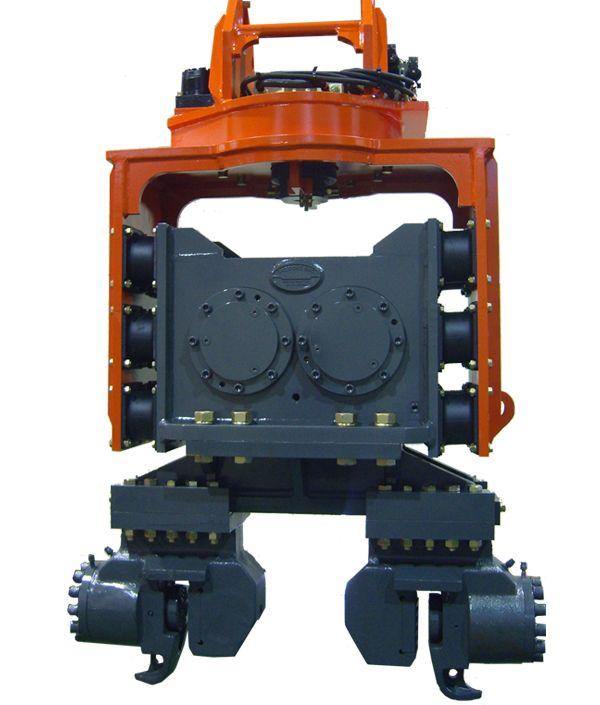
\includegraphics[width=1\linewidth]{../img/photo_1.jpg}
                    \end{figure}
                \end{minipage}
                \hfill
                \begin{minipage}[h]{0.22\linewidth}
                    \begin{figure}[h]
                        \centering
                        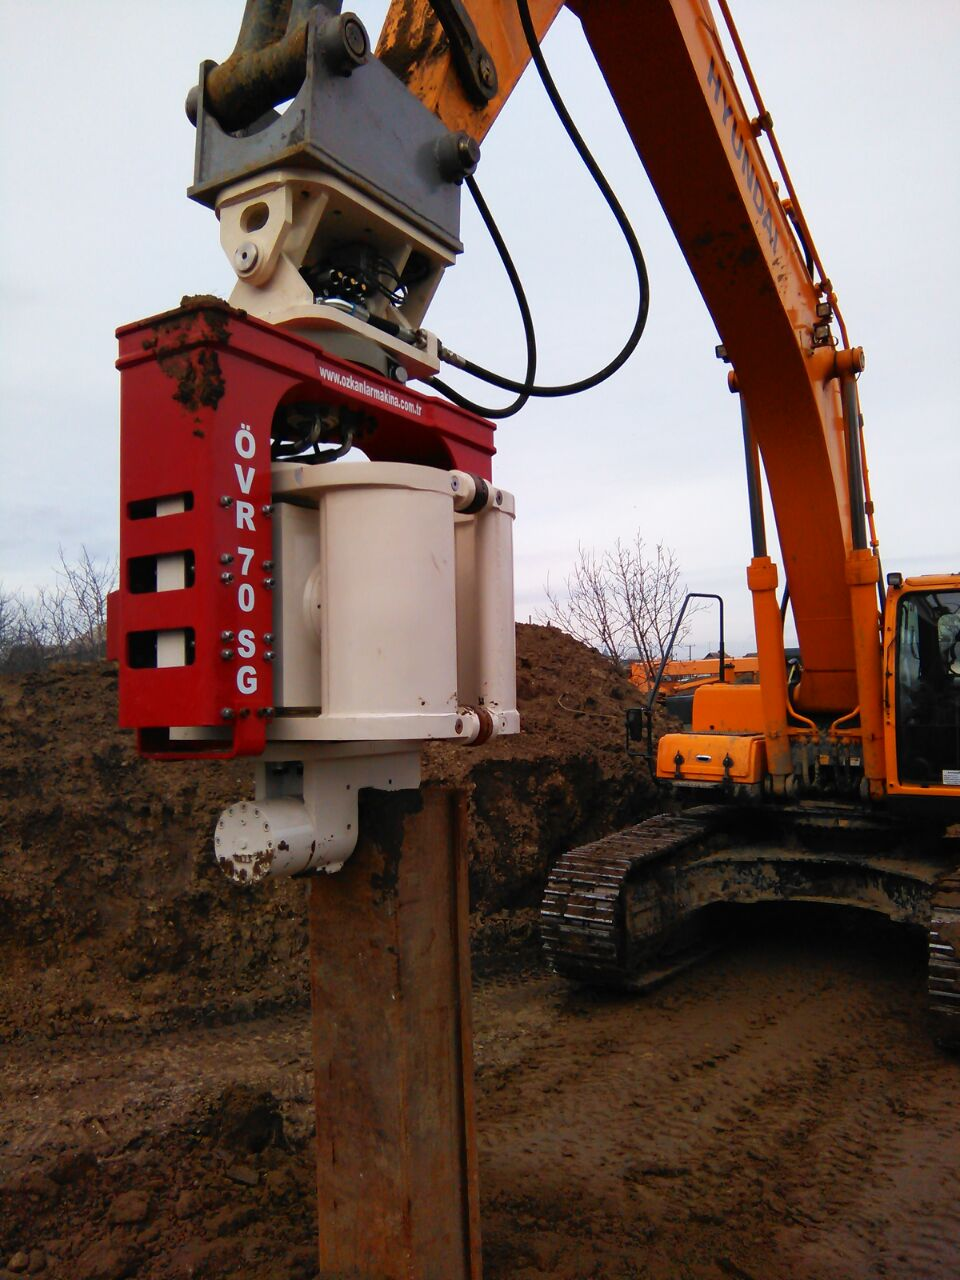
\includegraphics[width=1\linewidth]{../img/photo_2.jpg}
                    \end{figure}
                \end{minipage}
                \hfill
                \begin{minipage}[h]{0.29\linewidth}
                    \begin{figure}[h]
                        \centering
                        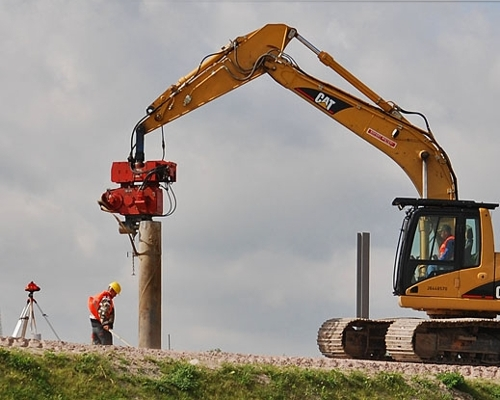
\includegraphics[width=1\linewidth]{../img/photo_3.jpg}
                    \end{figure}
                \end{minipage}
            \end{minipage}
        \end{center}
        \footnotetext[1]{\label{foot-1} Блехман И. И. Вибрационная механика. --- М. : Физико-математическая литература, 1994.}
        \footnotetext[2]{\label{foot-2} Костин Д. В. Бифуркация резонансных колебаний и оптимизация тригонометрического импульса по коэффициенту несимметрии // Математический сборник. --- М., 2016.}
    \end{frame}


    \begin{frame}
        \frametitle{Постановка задачи}
        \begin{center}
            \begin{minipage}[h]{0.97\linewidth}
                Для решения такой задачи необходимо на основе теории вибрационных машин и теоремы об оптимальности импульса Максвелла-Фейера
                разработать ПО для автоматизированного расчета характеристик импульсного погружателя
                с возможностью ввода начальных данных и наглядного вывода результатов.
            \end{minipage}
        \end{center}
    \end{frame}


    \begin{frame}
        \frametitle{Конструкция импульсного погружателя}
        \begin{center}
            \begin{minipage}[h]{0.97\linewidth}
                \begin{minipage}[h]{0.55\linewidth}
                    Работа погружателя основана на двух основных принципах:
                    \begin{enumerate} 
                        \item На эффекте резкого снижения сопротивлению погружения свайного элемента при сообщении последнему вибрации;
                        \item На действии полигармонического импульса, создаваемого центробежными силами системы дебалансов.
                    \end{enumerate}
                    При вращении валов (1) с дебалансами (2) на их ось крепления действует центробежная сила и погружатель получает вибрирующее движение,
                    которое через наголовник (3) сообщается свайному элементу (4).
                \end{minipage}
                \hfill
                \begin{minipage}[h]{0.36\linewidth}
                    \begin{figure}[h]
                        \centering
                        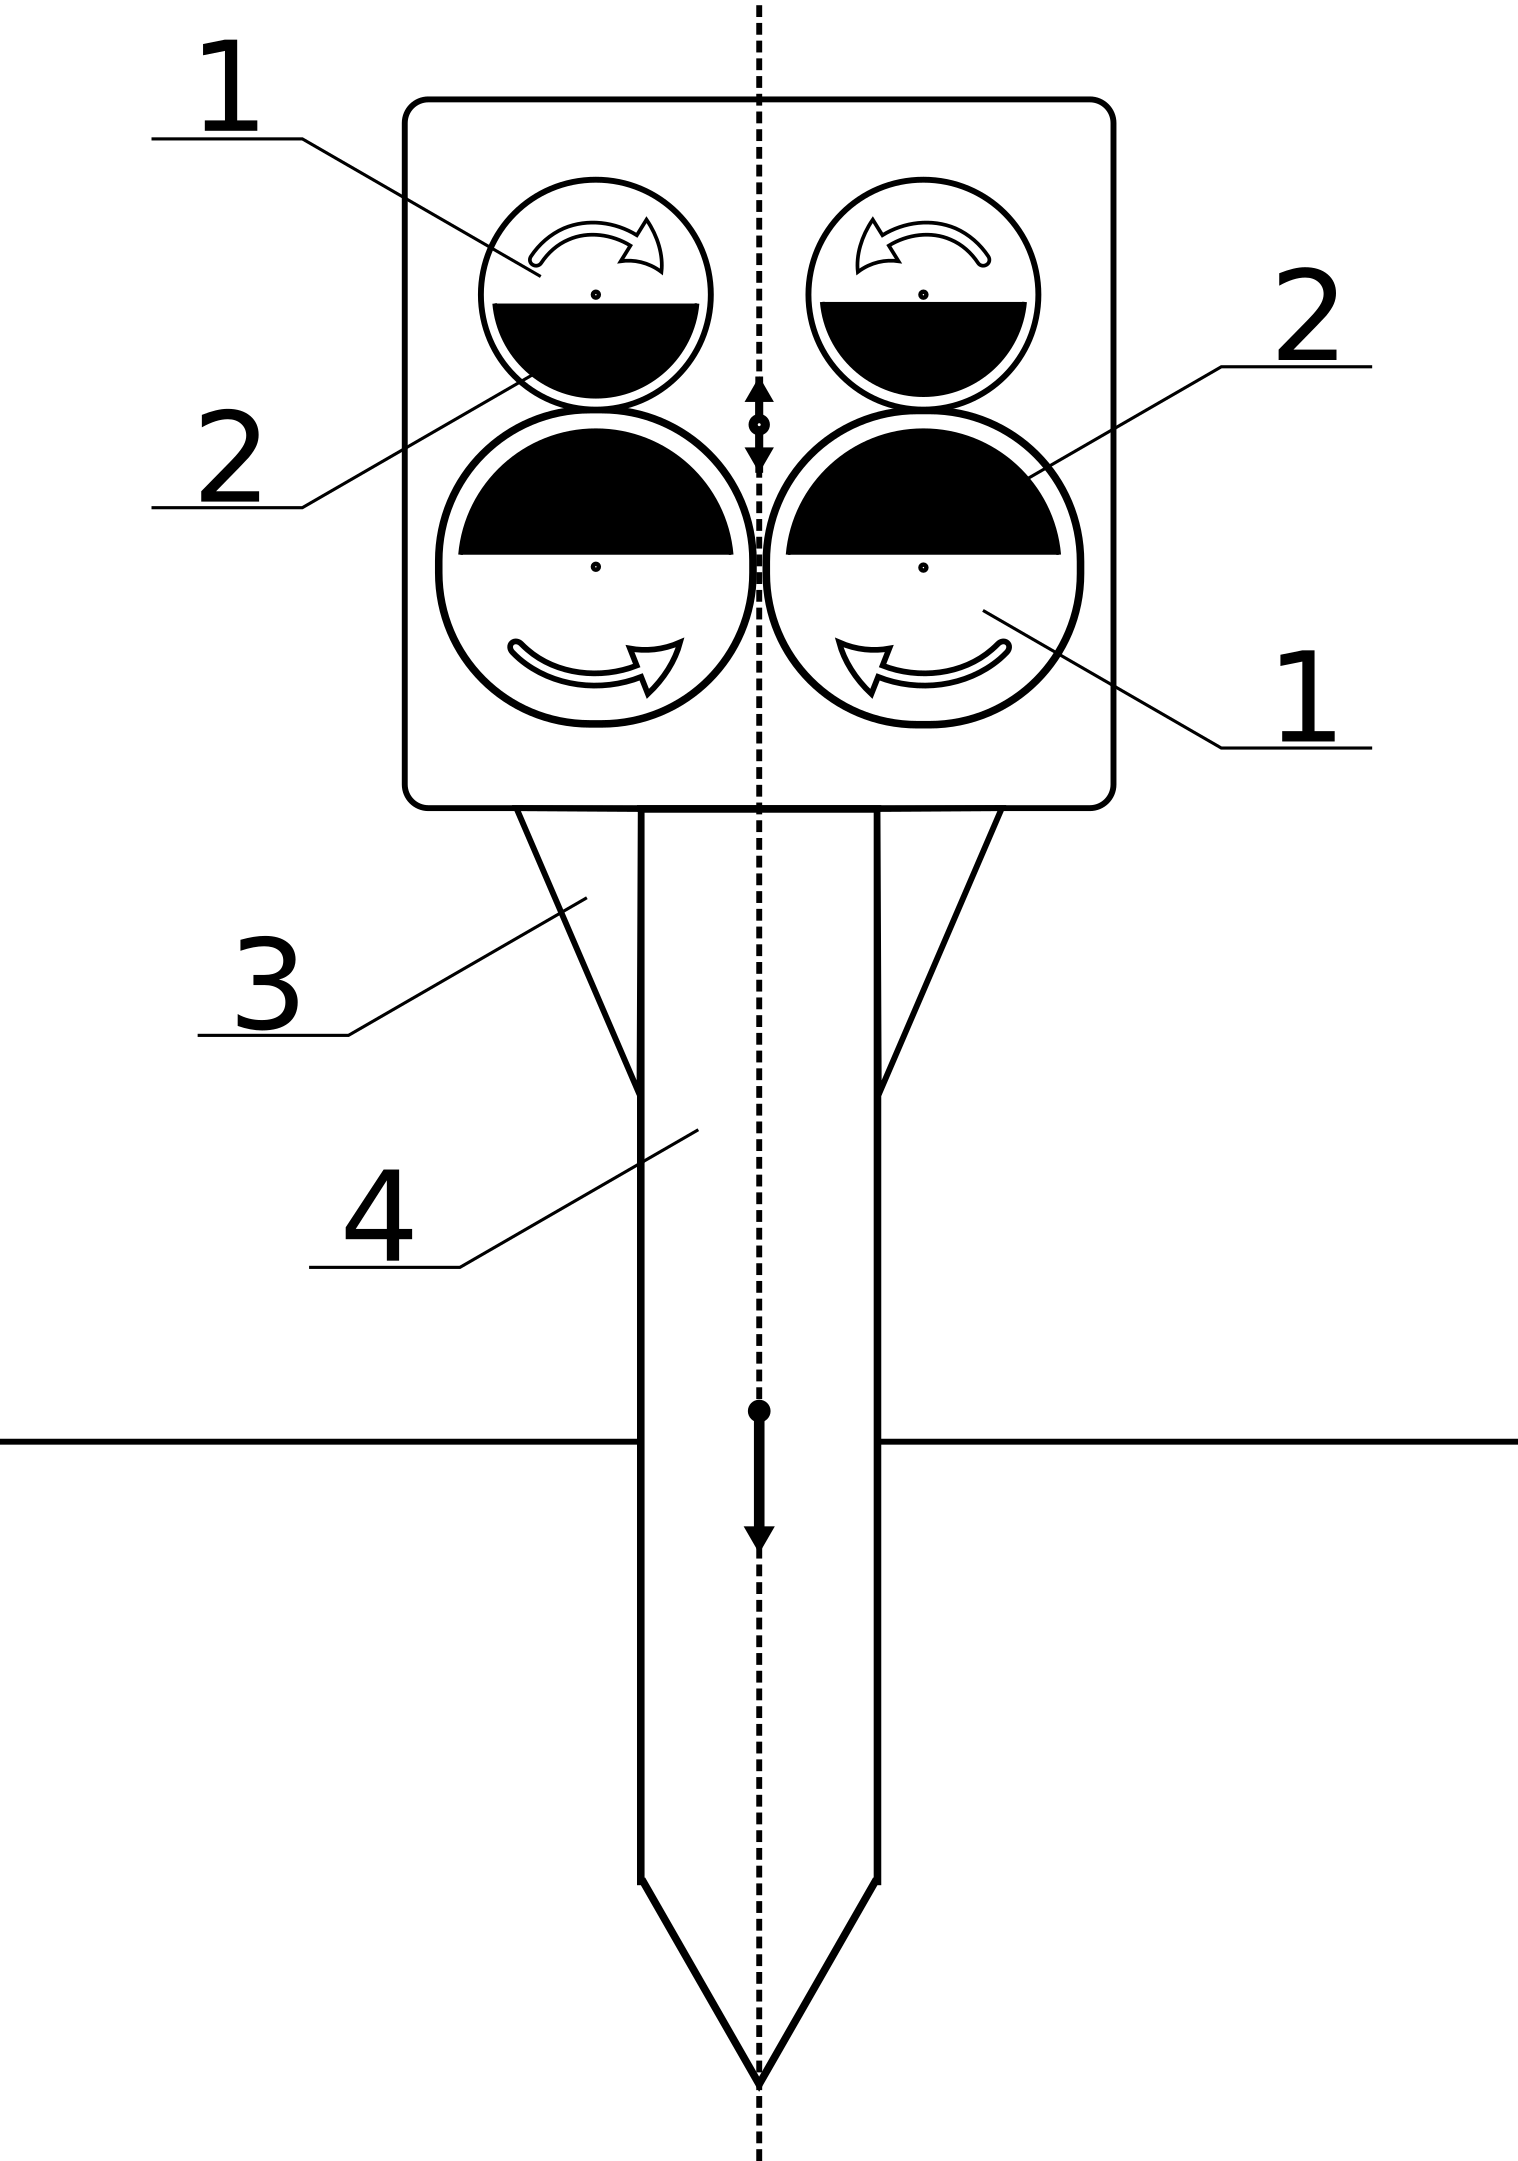
\includegraphics[width=1\linewidth]{../img/scheme_porg_2.png}
                        \caption{Схема импульсного погружателя.}
                    \end{figure}
                \end{minipage}
            \end{minipage}
        \end{center}
    \end{frame}


    \begin{frame}
        \frametitle{Конструкция дебаланса}
        \begin{center}
            \begin{minipage}[h]{0.97\linewidth}
                \begin{minipage}[h]{0.6\linewidth}
                    Пусть дан  дебаланс с радиусом $r$, радиус вала которого равен $R$,
                    $\omega$ --- угловая скорость и $l$ --- расстояние от центра масс до оси вращения дебаланса, а его масса будет равна $m$.
                    Центробежная сила:
                    \begin{equation}
                        \begin{gathered}
                            F_{\textrm{центр.}} = m \cdot \omega^2 \cdot l \\
                            \textrm{где } l = \frac{4 r}{3 \pi}
                        \end{gathered}
                    \end{equation}
                    \\
                    Гармонические колебания:
                    \begin{equation}
                        \begin{gathered}
                            x(t) = \lambda \cos (\omega t) \\
                            \textrm{где } \lambda = m \cdot \omega^2 \cdot l
                        \end{gathered}
                    \end{equation}
                \end{minipage}
                \hfill
                \begin{minipage}[h]{0.36\linewidth}
                    \begin{figure}[h]
                        \centering
                        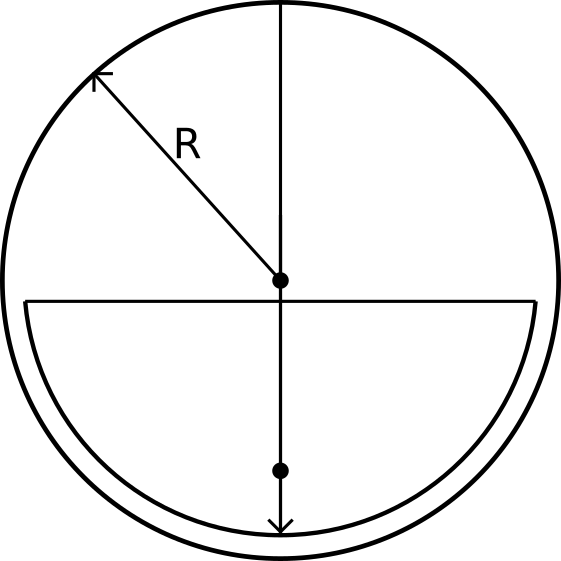
\includegraphics[width=1\linewidth]{../img/debalance.png}
                        \caption{Схема дебаланса.}
                    \end{figure}
                \end{minipage}
            \end{minipage}
        \end{center}
    \end{frame}


    \begin{frame}
        \frametitle{Конструкция пары дебалансов}
        \begin{center}
            \begin{minipage}[h]{0.97\linewidth}
                Для компенсации горизонтальных сил в конструкции погружателя используются парные дебалансы.\\
                Гармонические колебания пары дебалансов:
                \begin{equation}
                    \begin{gathered}
                        x(t) = 2 \lambda \cos (\omega t), \textrm{где } \lambda = m \cdot \omega^2 \cdot l
                    \end{gathered}
                \end{equation}
                \begin{figure}[h]
                    \centering
                    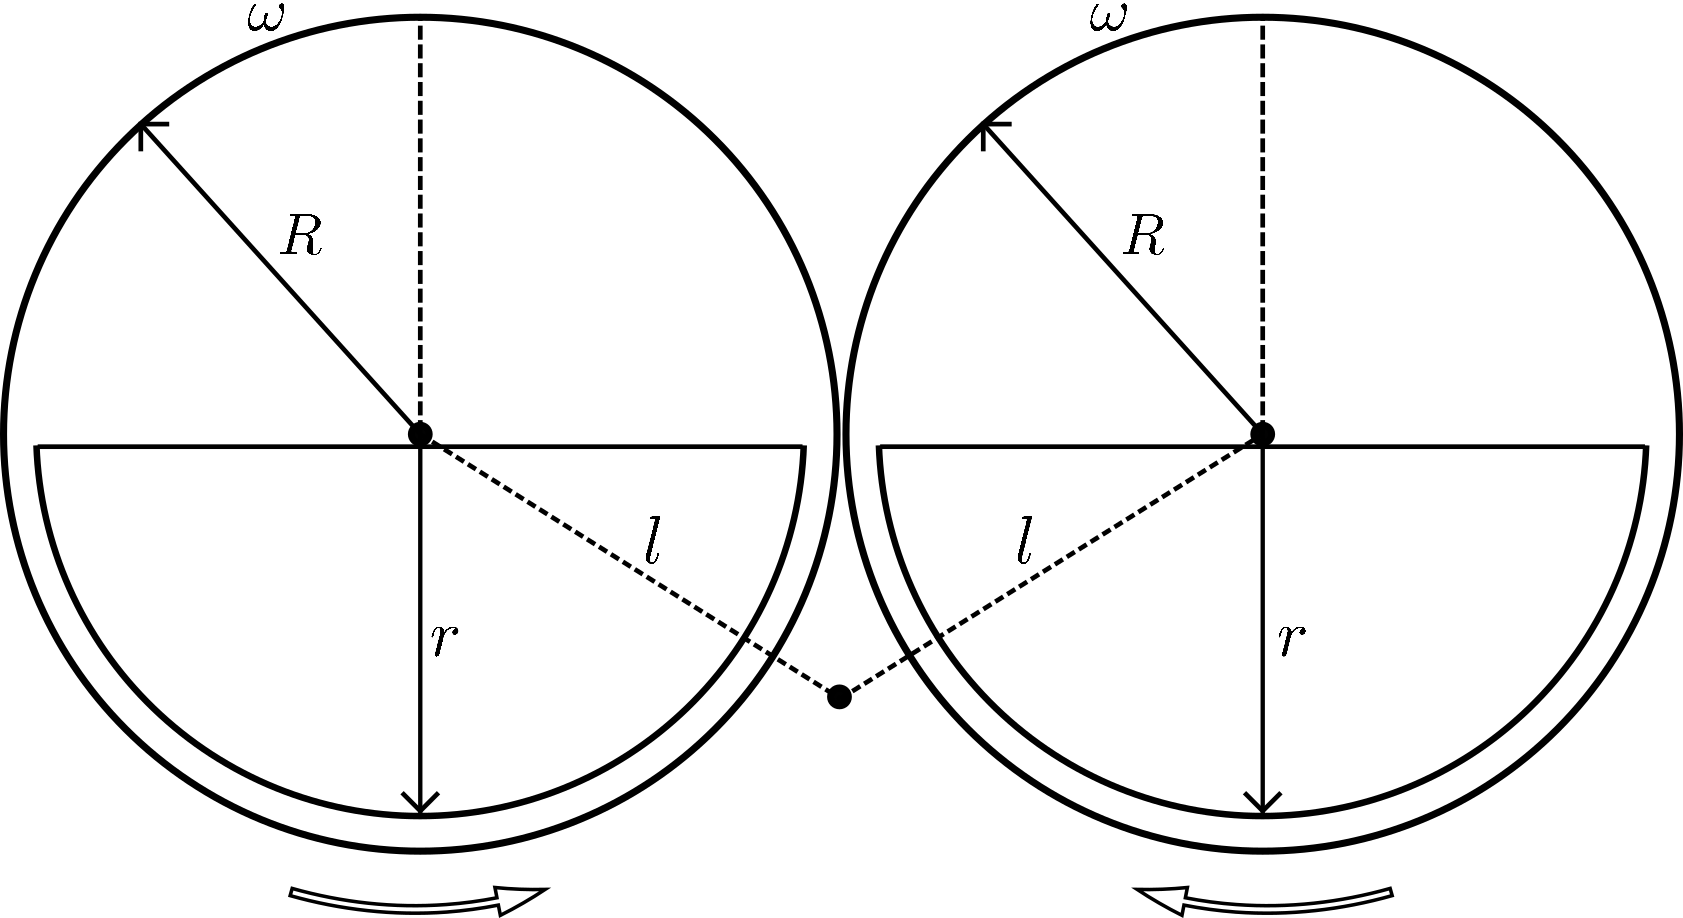
\includegraphics[width=0.52\linewidth]{../img/double_debalance.png}
                    \caption{Схема пары дебалансов.}
                \end{figure}
            \end{minipage}
        \end{center}
    \end{frame}


    \begin{frame}
        \frametitle{Гармонические колебания дебалансов}
        \begin{center}
            \begin{minipage}[h]{0.97\linewidth}
                При использовании нескольких пар дебалансов, вышестоящий уровень дебалансов должен иметь угловую скорость в два раза выше, чем прошлый.\\
                \newline
                \begin{minipage}[h]{0.44\linewidth}
                    \begin{figure}[h]
                        \centering
                        $x(t) = \lambda_1 \cos (\omega t)$
                        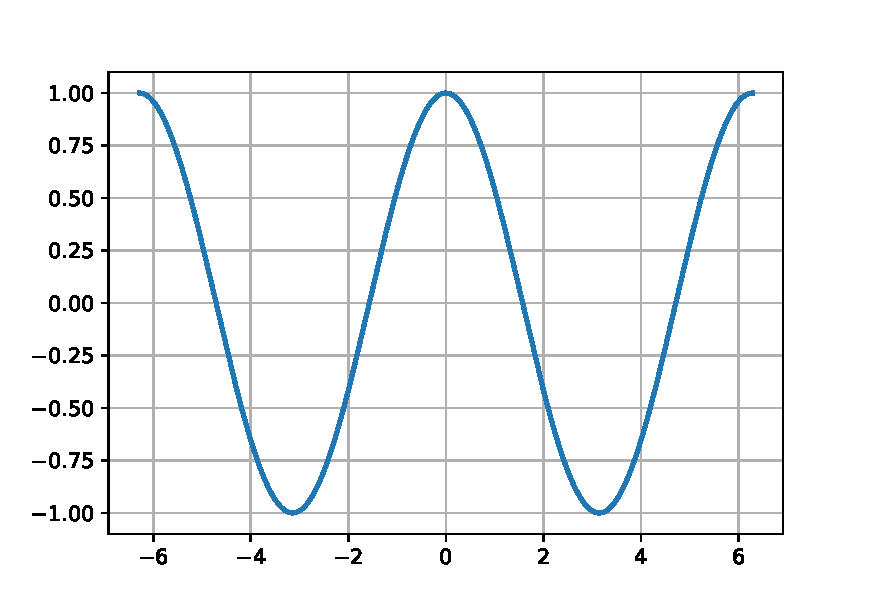
\includegraphics[width=1\linewidth]{../grap/impulse_1.pdf}
                        \caption{Гармонические колебания для одной пары дебалансов.}
                    \end{figure}
                \end{minipage}
                \hfill
                \begin{minipage}[h]{0.44\linewidth}
                    \begin{figure}[h]
                        \centering
                        $x(t) = \lambda_1 \cos (\omega t) + \lambda_2 \cos (2\omega t)$
                        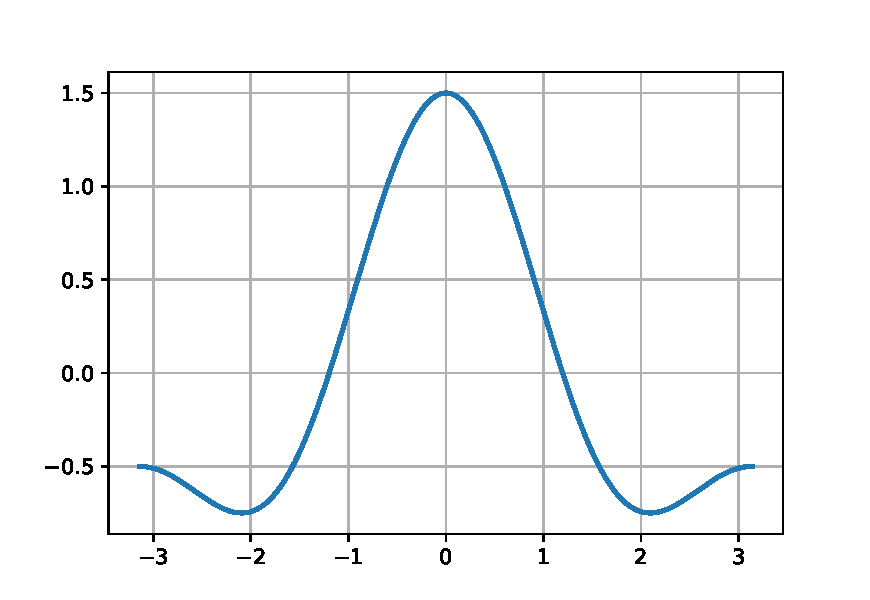
\includegraphics[width=1\linewidth]{../grap/impulse_2.pdf}
                        \caption{Гармонические колебания для двух пар дебалансов.}
                    \end{figure}
                \end{minipage}
            \end{minipage}
        \end{center}
    \end{frame}

    \begin{frame}
        \frametitle{Гармонические нескольких пар дебалансов}
        \begin{center}
            \begin{minipage}[h]{0.97\linewidth}
                Гармоническое колебания для $n$ дебалансов, где $k$ --- порядковый номер пары дебалансов, будет иметь вид:
                \begin{equation}\label{eq:harmonic_sum}
                    \begin{gathered}
                        F = \sum\limits_{k = 1}^n 2 \lambda_k \cdot \cos (k \omega t), \lambda = m \cdot \omega^2 \cdot l
                    \end{gathered}
                \end{equation}
                Использование нескольких пар дебалансов разных характеристик позволяет увеличить импульс,
                направленный на погружение свайного элемента и уменьшить импульс, направленный в противоположную сторону.
            \end{minipage}
        \end{center}
    \end{frame}


    \begin{frame}
        \frametitle{Задача оптимизации}
        \begin{center}
            \begin{minipage}[h]{0.97\linewidth}
                Пусть $f_{\max}(t)$ --- максимальное значение импульса силы за время $t$, $f_{\min}(t)$ --- минимальное значение импульса за время $t$. Тогда:
                \begin{equation}
                    \begin{gathered}
                        K = \left| \frac{f_{\max}(t)}{f_{\min}(t)} \right| \rightarrow \max
                    \end{gathered}
                \end{equation}
                \begin{block}{Теорема\footnotemark[3]}\label{teorema}
                    Многочлен (\ref{eq:harmonic_sum}) является оптимальным т. и т. т. , когда он с точностью до постоянного множителя имеет вид суммы Фейера:
                    \begin{equation}\label{eq:feer}
                        \begin{gathered}
                            f_n(t) = \sum\limits_{k = 1}^n (n + 1 - k) \cos(kt)\\
                            \max \limits_{\lambda} K_n(\lambda) = n
                        \end{gathered}
                    \end{equation}
                \end{block}
            \end{minipage}
        \end{center}
        \footnotetext[3]{\label{foot-3} Костин Д. В. Бифуркация резонансных колебаний и оптимизация тригонометрического импульса по коэффициенту несимметрии
        // Математический сборник. --- М., 2016. — С. 90—109.}
    \end{frame}

    \begin{frame}
        \frametitle{Задача оптимизации}
        \begin{center}
            \begin{minipage}[h]{0.97\linewidth}
                Исходя из теоремы выше, следует, что:
                \begin{equation}
                    \begin{gathered}
                        \lambda_k = \frac{n - k + 1}{n}
                    \end{gathered}
                \end{equation}
                Это позволяет найти коэффициент $\lambda$ для $k$-й пары дебалансов, когда общее количество дебалансов погружателя --- $n$.
            \end{minipage}
        \end{center}
    \end{frame}

    \begin{frame}
        \frametitle{Программная реализация}
        \begin{center}
            \begin{minipage}[h]{0.97\linewidth}
                При помощи применения теоремы об оптимальности модели полигармонического импульса и на основе теории вибрационных машин
                на языке Python была разработана программа для автоматического расчета характеристик дебалансов погружателя.
                \begin{figure}[h]
                    \centering
                    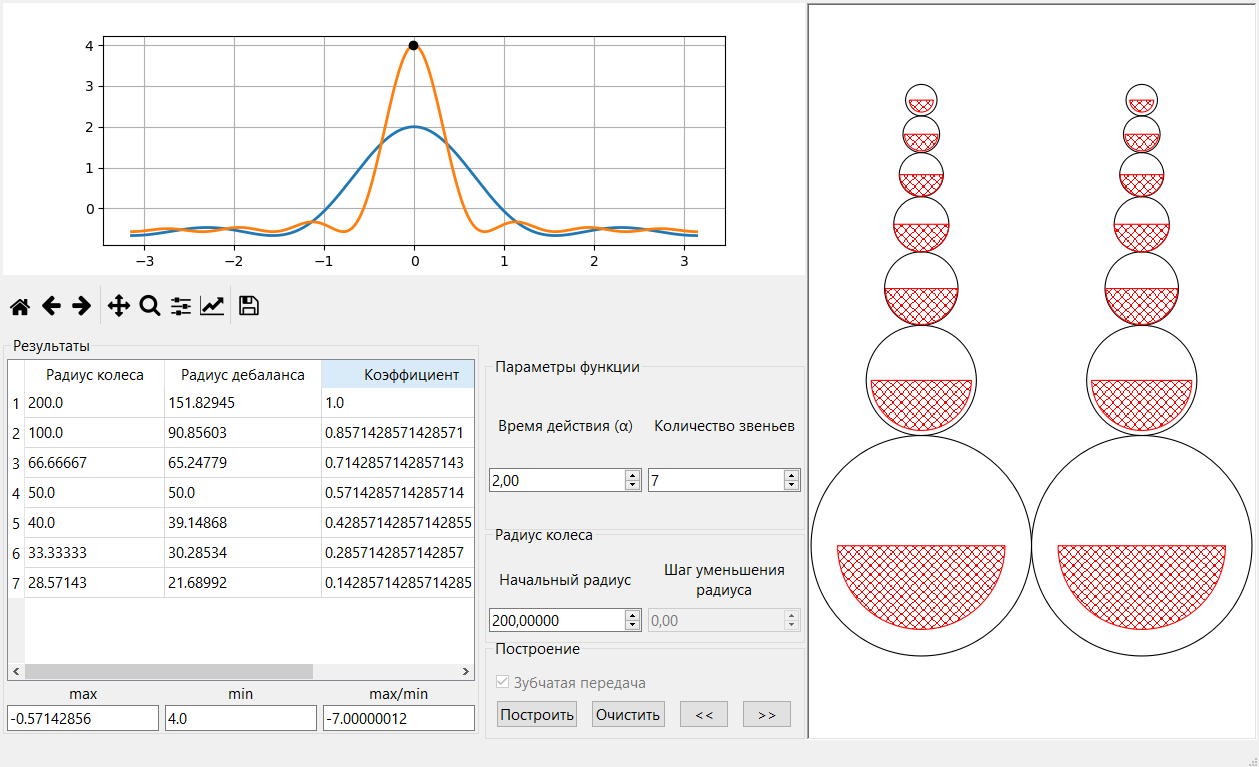
\includegraphics[width=0.62\linewidth]{../img/xolm_2.png}
                    \caption{Скриншот программы.}
                \end{figure}
            \end{minipage}
        \end{center}
    \end{frame}


    \begin{frame}
        \begin{alertblock}{}
            \centerline{\large Спасибо за внимание!}
        \end{alertblock}
    \end{frame}
\end{document}
